\section{单周期处理器}
\label{sec:04-processor-core-01}

% TODO：撰写本节正文。建议结构：
%   1) 问题引入与学习目标
%   2) 原理与机制（配图、公式）
%   3) 示例或实验步骤
%   4) 小结与思考题
本节待撰写。

\begin{figure}[htbp]
\centering
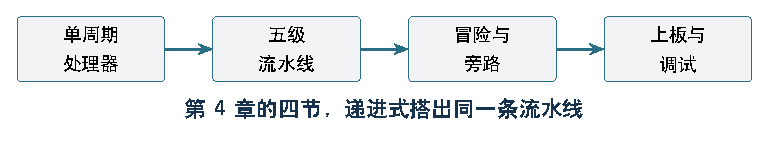
\includegraphics[width=.92\linewidth]{figures/chapter-overview}
\caption{第 4 章的四节：逐层搭出同一条流水线}
\label{fig:04-chapter-overview}
\end{figure}

全书主线（见\cref{fig:system-stack}）落到这一章，就是上面这条递进路径。

\begin{figure}[htbp]
\centering
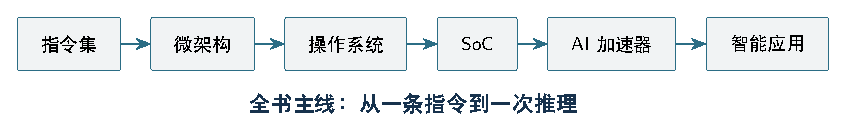
\includegraphics[width=\linewidth]{../01-system-overview/figures/system-stack}
\caption{跨章复用的图：这张图放在第 1 章，第 4 章直接引用同一个文件}
\label{fig:04-system-stack}
\end{figure}
